% =============================================================================
% Chiller Array Simulation Package — Technical Report
% =============================================================================
% Compile with: pdflatex report.tex && biber report && pdflatex report.tex && pdflatex report.tex
% Requires: amsmath, tikz, pgfplots, biblatex, algorithm2e, booktabs, listings
% =============================================================================

\documentclass[11pt, a4paper]{article}

% --- Page Layout ---
\usepackage[margin=1in]{geometry}

% --- Mathematics ---
\usepackage{amsmath, amssymb, amsthm}

% --- Graphics and Diagrams ---
\usepackage{tikz}
\usepackage{pgfplots}
\pgfplotsset{compat=1.18}
\usetikzlibrary{
    arrows.meta,
    positioning,
    shapes.geometric,
    calc,
    fit,
    backgrounds,
    decorations.pathmorphing
}

% --- Tables ---
\usepackage{booktabs}
\usepackage{array}

% --- References ---
\usepackage[backend=biber, style=numeric-comp, sorting=none]{biblatex}
\addbibresource{references.bib}

% --- Algorithms ---
\usepackage[ruled, vlined, linesnumbered]{algorithm2e}

% --- Code Listings ---
\usepackage{listings}
\lstset{
    language=Python,
    basicstyle=\ttfamily\small,
    keywordstyle=\bfseries,
    commentstyle=\itshape\color{gray},
    columns=flexible,
    breaklines=true,
    frame=single,
    xleftmargin=1em,
    framexleftmargin=0.5em,
}

% --- Typography ---
\usepackage{microtype}
\usepackage[colorlinks=true, linkcolor=blue!70!black, citecolor=blue!70!black, urlcolor=blue!70!black]{hyperref}
\usepackage{cleveref}

% --- Custom Commands ---
\newcommand{\cop}{\mathrm{COP}}
\newcommand{\copbase}{\cop_{\mathrm{base}}}
\newcommand{\dlong}{d_{\mathrm{long}}}
\newcommand{\dlat}{d_{\mathrm{lat}}}
\newcommand{\vwind}{\mathbf{w}}

% --- Title ---
\title{%
    \textbf{Chiller Array Simulation Package} \\[0.4em]
    \large Physics-Based Thermal Interference Modeling \\
    and Wind-Aware Optimization for Data Centers%
}
\author{Chiller Model Team}
\date{\today}

% =============================================================================
\begin{document}
% =============================================================================

\maketitle

% --- Abstract ---
\begin{abstract}
Densely packed chiller arrays in data centers suffer from thermal recirculation, where hot exhaust from one unit enters the intake of neighbouring units, degrading their Coefficient of Performance (COP).
This report describes \texttt{chiller-sim}, an open-source Python package that models these thermal interference effects using a Gaussian plume dispersion framework and provides greedy optimization tools for selecting the most energy-efficient subset of chillers to operate.
The package employs a modular, composition-based architecture with immutable thermodynamic states, validated inputs via Pydantic, and fully vectorized NumPy computations.
Simulation results indicate that thermal interference can reduce individual chiller COP by over 30\%, and that wind-aware optimization of chiller activation patterns can yield energy savings of 10--15\%.
Full documentation and examples are available at \url{https://chiller-model.readthedocs.io/}.
\end{abstract}

% =============================================================================
\section{Introduction}
\label{sec:introduction}
% =============================================================================

Modern data centers require substantial cooling capacity to dissipate the thermal load produced by servers and networking equipment.
Air-cooled chiller arrays, which reject heat to the outdoor ambient air, are a common solution~\cite{cho2014datacenter}.
When these chillers are deployed in dense configurations, a phenomenon known as \emph{thermal recirculation} can arise~\cite{ashrae2020hvac}.
In this scenario, the hot exhaust plume discharged by one chiller drifts downwind and is partially ingested by adjacent units, effectively raising their condenser inlet temperature.

The consequences of this effect are significant.
An elevated inlet temperature forces the compressor to work harder to achieve the same cooling capacity, thereby reducing the Coefficient of Performance (COP).
Field observations and simulations suggest that individual chiller COP can degrade by more than 30\% under unfavourable wind conditions~\cite{ashrae2019applications}.
Yet not all configurations suffer equally: the magnitude of thermal interference depends on the arrangement of units, the prevailing wind direction, and the number of chillers operating simultaneously.

The \texttt{chiller-sim} package addresses this problem by providing a physics-based simulation framework that captures thermal interference through Gaussian plume dispersion theory~\cite{pasquill1961estimation, gifford1961turbulent}.
In addition to modelling COP degradation, the package includes a greedy optimization algorithm that identifies which chillers to activate in order to minimise total electrical consumption for a given cooling load.
Key design findings include the counter-intuitive result that operating \emph{fewer} chillers can sometimes be more efficient than running the entire array, since deactivating certain units eliminates the thermal penalty they impose on their neighbours.

The remainder of this report is organized as follows:
\Cref{sec:mathematical-formulation} presents the mathematical formulation, including the Gaussian plume model and COP degradation equations.
\Cref{sec:architecture} describes the software architecture and its design principles.
\Cref{sec:optimization} details the greedy optimization algorithm.
\Cref{sec:results} provides representative simulation results and discusses validation against the AHRI~550/590 standard.
Finally, \Cref{sec:conclusion} summarizes the main contributions and outlines future directions.

% =============================================================================
\section{Mathematical Formulation}
\label{sec:mathematical-formulation}
% =============================================================================

This section develops the mathematical model that underpins the simulation.
All internal computations use SI units: temperatures in Kelvin, distances in meters, power in kilowatts, and pressures in Pascals~\cite{ashrae2021fundamentals}.

% --- 2.1 Problem Setup ---
\subsection{Problem Setup}
\label{sec:problem-setup}

Consider an array of $N$ chillers positioned in a two-dimensional plane.
Each chiller $m$ occupies position $\mathbf{p}_m = (x_m, y_m)$ in meters.
A uniform wind field is characterized by velocity vector $\vwind = (w_x, w_y)$ in m/s, with unit direction $\hat{\vwind} = \vwind / \|\vwind\|$.
Every chiller shares a common base COP, denoted $\copbase$, and a temperature sensitivity coefficient $\alpha$.
The total cooling load $Q_{\mathrm{total}}$ (kW) must be distributed among the active chillers.

% --- 2.2 Distance Decomposition ---
\subsection{Distance Decomposition}
\label{sec:distance-decomposition}

For each pair of chillers $(k, m)$, the displacement vector from $k$ to $m$ is
\begin{equation}
    \label{eq:displacement}
    \mathbf{d}_{km} = \mathbf{p}_m - \mathbf{p}_k.
\end{equation}
This vector is decomposed into components parallel and perpendicular to the wind direction.
The \emph{longitudinal distance} (along the wind) is obtained by projection:
\begin{equation}
    \label{eq:longitudinal}
    \dlong^{(km)} = \mathbf{d}_{km} \cdot \hat{\vwind}.
\end{equation}
A positive value of $\dlong^{(km)}$ indicates that chiller $m$ is downwind of chiller $k$.
The \emph{lateral distance} (perpendicular to the wind) follows from vector subtraction:
\begin{equation}
    \label{eq:lateral}
    \dlat^{(km)} = \bigl\| \mathbf{d}_{km} - \dlong^{(km)} \hat{\vwind} \bigr\|.
\end{equation}

% --- 2.3 Gaussian Plume Model ---
\subsection{Gaussian Plume Interaction Model}
\label{sec:gaussian-plume}

The thermal impact of chiller $k$ on chiller $m$ is modeled using a Gaussian plume dispersion kernel~\cite{pasquill1961estimation, epa1995ap42}:
\begin{equation}
    \label{eq:plume}
    \boxed{\;
    A_{km} = \frac{\exp\!\Bigl(-\dfrac{(\dlat^{(km)})^2}{\;\sigma\,(\dlong^{(km)} + 1)\;}\Bigr)}{\dlong^{(km)} + 1}
    \;}
\end{equation}
where $\sigma > 0$ is the dispersion coefficient that controls the rate of lateral plume spread.
Larger values of $\sigma$ correspond to faster dispersion and therefore weaker thermal interference.
The additive constant of 1 in the denominator serves as a regularization term that prevents singularities when two chillers are positioned very close together.

Three physical constraints are enforced on the interaction matrix $\mathbf{A} \in \mathbb{R}^{N \times N}$:
\begin{enumerate}
    \item \textbf{No self-interaction}: $A_{mm} = 0$ for all $m$.
    \item \textbf{Downwind only}: $A_{km} = 0$ whenever $\dlong^{(km)} \leq 0$, since upwind units do not receive exhaust from chiller $k$.
    \item \textbf{Non-negativity}: $A_{km} \geq 0$ for all $(k, m)$.
\end{enumerate}

The exponential term in~\eqref{eq:plume} represents the Gaussian lateral decay of the thermal plume, while the factor $1/(\dlong^{(km)} + 1)$ captures the longitudinal dilution as the plume travels downwind.
Together, they encode the physical intuition that nearby, directly-downwind chillers experience the strongest interference, and that lateral offset reduces the impact exponentially.

% --- Visualization of Gaussian Plume ---
\begin{figure}[htbp]
    \centering
    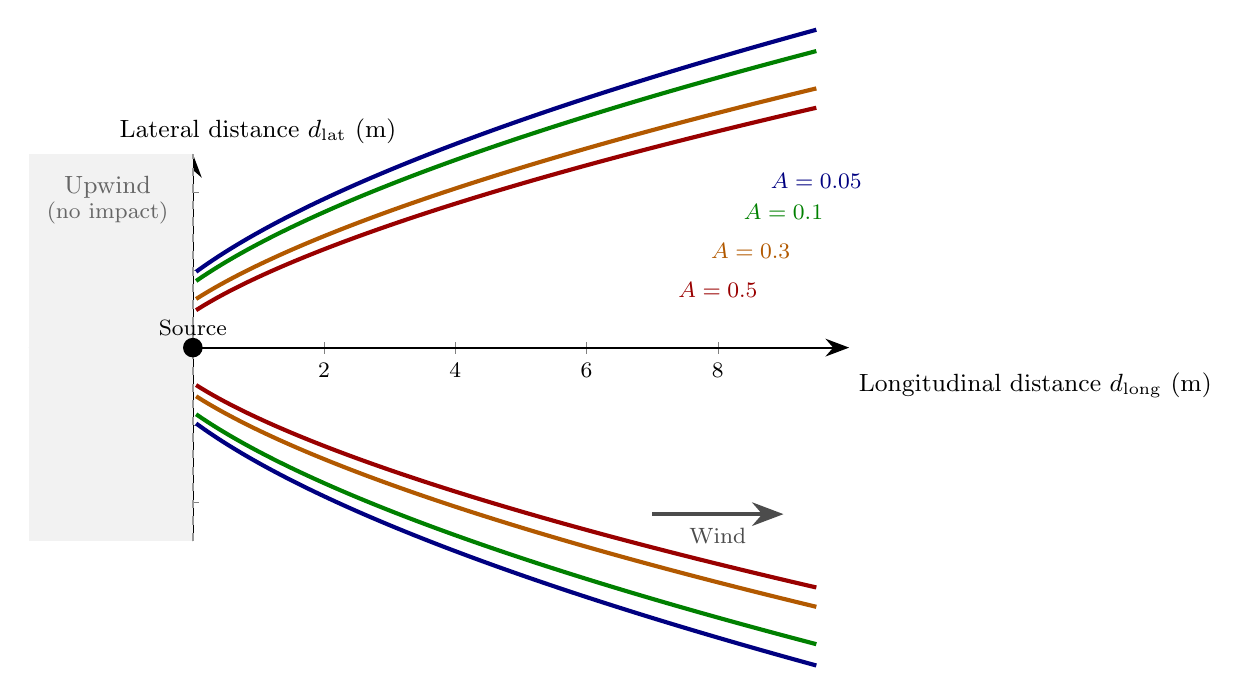
\begin{tikzpicture}
        \begin{axis}[
            width=12cm,
            height=6.5cm,
            xlabel={Longitudinal distance $\dlong$ (m)},
            ylabel={Lateral distance $\dlat$ (m)},
            xmin=-2.5, xmax=10,
            ymin=-5, ymax=5,
            axis lines=center,
            axis line style={-{Stealth[length=3mm]}, thick},
            xlabel style={at={(axis description cs:1.0,0.46)}, anchor=north west, font=\small},
            ylabel style={at={(axis description cs:0.46,1.0)}, anchor=south east, font=\small},
            xtick={-2,0,2,4,6,8},
            ytick={-4,-2,0,2,4},
            tick label style={font=\footnotesize},
            clip=false,
        ]
            % Upwind region (no impact, shaded)
            \fill[black!5] (axis cs:-2.5,-5) rectangle (axis cs:0,5);
            
            % Cutoff line at x=0
            \draw[black!40, thick, dashed] (axis cs:0,-5) -- (axis cs:0,5);
            
            % Level set contours (calculated for sigma=1.2)
            % A = exp(-d_lat^2 / (sigma*(d_long+1))) / (d_long+1)
            
            \addplot[red!60!black, line width=1.5pt, smooth, domain=0.05:9.5, samples=150] 
                ({x}, {sqrt(1.2*(x+1)*ln((x+1)/0.5))});
            \addplot[red!60!black, line width=1.5pt, smooth, domain=0.05:9.5, samples=150] 
                ({x}, {-sqrt(1.2*(x+1)*ln((x+1)/0.5))});
            
            \addplot[orange!70!black, line width=1.5pt, smooth, domain=0.05:9.5, samples=150] 
                ({x}, {sqrt(1.2*(x+1)*ln((x+1)/0.3))});
            \addplot[orange!70!black, line width=1.5pt, smooth, domain=0.05:9.5, samples=150] 
                ({x}, {-sqrt(1.2*(x+1)*ln((x+1)/0.3))});
            
            \addplot[green!50!black, line width=1.5pt, smooth, domain=0.05:9.5, samples=150] 
                ({x}, {sqrt(1.2*(x+1)*ln((x+1)/0.1))});
            \addplot[green!50!black, line width=1.5pt, smooth, domain=0.05:9.5, samples=150] 
                ({x}, {-sqrt(1.2*(x+1)*ln((x+1)/0.1))});
            
            \addplot[blue!50!black, line width=1.5pt, smooth, domain=0.05:9.5, samples=150] 
                ({x}, {sqrt(1.2*(x+1)*ln((x+1)/0.05))});
            \addplot[blue!50!black, line width=1.5pt, smooth, domain=0.05:9.5, samples=150] 
                ({x}, {-sqrt(1.2*(x+1)*ln((x+1)/0.05))});
            
            % Source chiller at origin
            \node[circle, fill=black, inner sep=2.5pt] at (axis cs:0,0) {};
            \node[font=\footnotesize, above=1pt] at (axis cs:0,0) {Source};
            
            % Labels for level sets (positioned to avoid overlap)
            \node[font=\footnotesize, red!60!black] at (axis cs:8, 1.5) {$A=0.5$};
            \node[font=\footnotesize, orange!70!black] at (axis cs:8.5, 2.5) {$A=0.3$};
            \node[font=\footnotesize, green!50!black] at (axis cs:9, 3.5) {$A=0.1$};
            \node[font=\footnotesize, blue!50!black] at (axis cs:9.5, 4.3) {$A=0.05$};
            
            % Upwind label
            \node[font=\small, black!60, align=center] at (axis cs:-1.3, 3.8) {Upwind\\[-2pt]{\footnotesize (no impact)}};
            
            % Wind direction arrow
            \draw[-{Stealth[length=4mm]}, line width=1.2pt, black!70] 
                (axis cs:7, -4.3) -- (axis cs:9, -4.3) 
                node[midway, below=1pt, font=\footnotesize] {Wind};
        \end{axis}
    \end{tikzpicture}
    \caption{Gaussian plume dispersion model for thermal interference ($\sigma = 1.2$).
    Level sets show contours of constant impact $A_{km}$.
    The source chiller is at the origin.
    Shaded region ($\dlong \leq 0$) represents the upwind zone with zero thermal impact.
    The plume expands laterally with Gaussian decay while diminishing longitudinally as $1/(\dlong + 1)$.}
    \label{fig:gaussian-plume}
\end{figure}

% --- 2.4 COP Degradation ---
\subsection{COP Degradation}
\label{sec:cop-degradation}

The cumulative thermal interference at chiller $m$ is obtained by summing the contributions of all active chillers.
Let $s_k \in \{0, 1\}$ denote the activation state of chiller $k$.
The effective temperature rise at the inlet of chiller $m$ is
\begin{equation}
    \label{eq:temp-rise}
    \Delta T_m = \sum_{k=1}^{N} A_{km} \, s_k.
\end{equation}
The degraded COP at chiller $m$ then follows the inverse-linear model~\cite{ashrae2020hvac}:
\begin{equation}
    \label{eq:cop-degradation}
    \boxed{\;
    \cop_m = \frac{\copbase}{1 + \alpha \, \Delta T_m}
    \;}
\end{equation}
where $\alpha$ is the sensitivity coefficient that governs how strongly the COP responds to inlet temperature rise.
This model is based on the relationship between COP and the Carnot efficiency of the refrigeration cycle. In the Carnot efficiency equation, the inlet temperature of the hot side has a inverse linear relationship with the COP.
Calibrating this value may require field measurements or empirical data. Our default value for demonstration purposes is $\alpha = 0.7$~\cite{ashrae2019applications}.

% --- 2.5 Power Consumption ---
\subsection{Power Consumption and Load Distribution}
\label{sec:power-consumption}

For demonstration purposes, we assume the total cooling load $Q_{\mathrm{total}}$ is distributed evenly among the $n$ active chillers:
\begin{equation}
    \label{eq:load-distribution}
    Q_m = \frac{Q_{\mathrm{total}}}{n}, \qquad n = \sum_{k=1}^{N} s_k.
\end{equation}
The electrical power consumed by each active chiller is
\begin{equation}
    \label{eq:power}
    P_m = \frac{Q_m}{\cop_m},
\end{equation}
and the total system work is
\begin{equation}
    \label{eq:total-work}
    W_{\mathrm{total}} = \sum_{m=1}^{N} s_m \, P_m = \sum_{m=1}^{N} s_m \, \frac{Q_m}{\cop_m}.
\end{equation}
The effective system-level COP is defined as $\cop_{\mathrm{eff}} = Q_{\mathrm{total}} / W_{\mathrm{total}}$.

% --- 2.6 Parameter Table ---
\subsection{Default Parameters and Physical Bounds}
\label{sec:parameters}

\Cref{tab:parameters} summarizes the key model parameters andtheir demonstration values. These parameters will need to be calibrated for each specific application.

\begin{table}[htbp]
    \centering
    \caption{Model parameters and their demo values.}
    \label{tab:parameters}
    \begin{tabular}{@{}llll@{}}
        \toprule
        \textbf{Parameter} & \textbf{Symbol} & \textbf{Default} \\
        \midrule
        Base COP              & $\copbase$  & 4.0        \\
        Sensitivity coeff.    & $\alpha$    & 0.7        \\
        Dispersion coeff.     & $\sigma$    & 1.2        \\
        Ambient temperature   & $T_a$       & 298.15\,K   \\
        Standard pressure     & ---         & 101\,325\,Pa \\
        \bottomrule
    \end{tabular}
\end{table}

% =============================================================================
\section{Software Architecture}
\label{sec:architecture}
% =============================================================================

The package adopts a modular, composition-based architecture organized into three layers: layout, physics, and simulation.
This design follows the principle of composition over inheritance: the \texttt{Simulator} is constructed via a fluent \texttt{SimulatorBuilder} that composes a \texttt{ChillerGrid}, \texttt{WindConditions}, and pluggable physics functions rather than relying on class inheritance~\cite{ham2015dynamic}.

% --- TikZ Architecture Diagram ---
\begin{figure}[htbp]
    \centering
    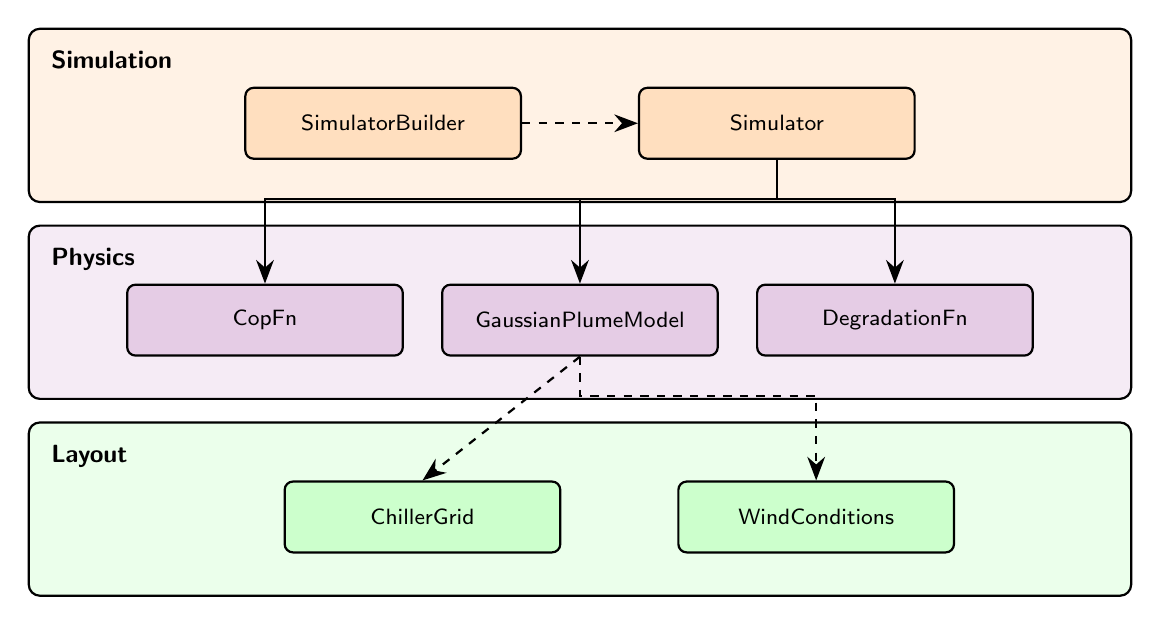
\begin{tikzpicture}[
        layer/.style={draw, rounded corners, minimum width=14cm, minimum height=2.2cm,
                      thick, font=\sffamily\small},
        block/.style={draw, rounded corners=3pt, minimum width=3.5cm, minimum height=0.9cm,
                      thick, font=\sffamily\footnotesize, text centered},
        arr/.style={-{Stealth[length=3mm]}, thick},
        darr/.style={-{Stealth[length=3mm]}, thick, dashed},
    ]
        % Simulation Layer
        \node[layer, fill=orange!10] (sim) at (0, 5.0) {};
        \node[anchor=north west, font=\sffamily\small\bfseries] at ([xshift=5pt, yshift=-5pt] sim.north west) {Simulation};
        \node[block, fill=orange!25] (builder) at (-2.5, 4.9) {SimulatorBuilder};
        \node[block, fill=orange!25] (simulator) at (2.5, 4.9) {Simulator};

        % Physics Layer
        \node[layer, fill=violet!8] (phys) at (0, 2.5) {};
        \node[anchor=north west, font=\sffamily\small\bfseries] at ([xshift=5pt, yshift=-5pt] phys.north west) {Physics};
        \node[block, fill=violet!20] (cop) at (-4, 2.4) {CopFn};
        \node[block, fill=violet!20] (gauss) at (0, 2.4) {GaussianPlumeModel};
        \node[block, fill=violet!20] (degrad) at (4, 2.4) {DegradationFn};

        % Layout Layer
        \node[layer, fill=green!8] (lay) at (0, 0.0) {};
        \node[anchor=north west, font=\sffamily\small\bfseries] at ([xshift=5pt, yshift=-5pt] lay.north west) {Layout};
        \node[block, fill=green!20] (grid) at (-2, -0.1) {ChillerGrid};
        \node[block, fill=green!20] (wind) at (3, -0.1) {WindConditions};

        % Arrows: Simulation -> Physics
        \draw[arr] (simulator.south) -- ++(0,-0.5) -| (cop.north);
        \draw[arr] (simulator.south) -- ++(0,-0.5) -| (gauss.north);
        \draw[arr] (simulator.south) -- ++(0,-0.5) -| (degrad.north);
        \draw[darr] (builder.east) -- (simulator.west);

        % Arrows: Physics -> Layout
        \draw[darr] (gauss.south) -- (grid.north);
        \draw[darr] (gauss.south) -- ++(0,-0.5) -| (wind.north);
    \end{tikzpicture}
    \caption{Layered architecture of the \texttt{chiller-sim} package.
    Solid arrows denote composition; dashed arrows denote dependency or extension.}
    \label{fig:architecture}
\end{figure}

Thermodynamic states are treated as immutable throughout the package.
The \texttt{ChillerGrid} class is implemented as a frozen dataclass, and result types (\texttt{OptimizeResult}, \texttt{SimulationResult}) use immutable structures.
Returning a new state object after each thermodynamic process eliminates an entire class of mutation-related bugs and simplifies reasoning about the simulation flow.

Input validation is handled by the \texttt{SimulatorBuilder}, which enforces required fields and physically plausible parameter ranges at build time.

All performance-critical computations are fully vectorized using NumPy~\cite{harris2020numpy}.
The interaction matrix $\mathbf{A}$ is computed in a single pass using broadcasting and \texttt{np.einsum} for the wind-direction projection, without any explicit Python-level loops.
This matrix is pre-computed at initialization and reused during optimization, where the same environment may be evaluated hundreds of times.

% =============================================================================
\section{Optimization Algorithm}
\label{sec:optimization}
% =============================================================================

Given a fixed cooling load, the optimization problem seeks the activation vector $\mathbf{s}^{*} \in \{0,1\}^N$ that minimizes total electrical work:
\begin{equation}
    \label{eq:optimization}
    \mathbf{s}^{*} = \arg\min_{\mathbf{s}} \; W_{\mathrm{total}}(\mathbf{s})
    \qquad \text{subject to} \quad \sum_{k} s_k \geq n_{\min}.
\end{equation}
Since this is a combinatorial problem with $2^N$ possible configurations, an exhaustive search is impractical for large arrays.
The package therefore employs a greedy removal heuristic, described in~\Cref{alg:greedy}.

\begin{algorithm}[htbp]
    \SetAlgoLined
    \KwIn{Environment $\mathcal{E}$, total load $Q_{\mathrm{total}}$, minimum active $n_{\min}$}
    \KwOut{Optimal activation mask $\mathbf{s}^{*}$}
    $\mathbf{s} \leftarrow \mathbf{1}_N$ \tcp*{Start with all chillers active}
    $W^{*} \leftarrow W_{\mathrm{total}}(\mathbf{s})$ \tcp*{Compute baseline work}
    \While{$\sum_k s_k > n_{\min}$}{
        $W_{\mathrm{best}} \leftarrow W^{*}$\;
        $j^{*} \leftarrow -1$\;
        \ForEach{active chiller $j$ where $s_j = 1$}{
            $\tilde{\mathbf{s}} \leftarrow \mathbf{s}$ with $\tilde{s}_j = 0$ \tcp*{Trial removal}
            $W_j \leftarrow W_{\mathrm{total}}(\tilde{\mathbf{s}})$\;
            \If{$W_j < W_{\mathrm{best}}$}{
                $W_{\mathrm{best}} \leftarrow W_j$\;
                $j^{*} \leftarrow j$\;
            }
        }
        \eIf{$j^{*} \geq 0$ \textbf{and} $W_{\mathrm{best}} < W^{*}$}{
            $s_{j^{*}} \leftarrow 0$ \tcp*{Apply best removal}
            $W^{*} \leftarrow W_{\mathrm{best}}$\;
        }{
            \textbf{break} \tcp*{No improvement; converged}
        }
    }
    \Return $\mathbf{s}$\;
    \caption{Greedy chiller removal algorithm.}
    \label{alg:greedy}
\end{algorithm}

The algorithm begins with all chillers active and iteratively removes the single chiller whose deactivation yields the greatest reduction in total work.
At each iteration, it evaluates all $n$ currently active chillers, computing the performance for each trial configuration.
This yields a per-iteration complexity of $\mathcal{O}(N^2)$, since each performance evaluation involves a matrix--vector product with the $N \times N$ interaction matrix.

Convergence is guaranteed because total work is bounded below by zero and each accepted removal strictly reduces work.
The algorithm terminates when one of three conditions is met: no single removal improves the objective, the minimum active count $n_{\min}$ has been reached, or a user-specified iteration limit is exhausted.
Although the greedy strategy does not guarantee a global optimum, it is effective in practice because the thermal interference structure typically exhibits strong spatial locality.

% =============================================================================
\section{Results and Validation}
\label{sec:results}
% =============================================================================

To illustrate the capabilities of the package, consider a $5 \times 5$ chiller array with 3\,m spacing, a base COP of 4.0, and a sensitivity coefficient $\alpha = 0.7$.
Wind blows with velocity vector $(1.0, 0.4)$\,m/s at an ambient temperature of 298.15\,K (25\,\textdegree{}C).
The dispersion coefficient is set to $\sigma = 1.2$.

\Cref{fig:thermal-plume-actual} shows the thermal wake effect from a single source chiller (center unit) in this configuration.
The colormap illustrates how thermal interference propagates primarily in the downwind direction, with intensity decaying both laterally and longitudinally according to the Gaussian plume model.

\begin{figure}[htbp]
    \centering
    \includegraphics[width=0.75\textwidth]{figure_1_thermal_plume.png}
    \caption{Thermal wake visualization showing the impact of a single source chiller on neighboring units in a $5 \times 5$ array.
    The wind vector $(1.0, 0.4)$\,m/s determines the direction and intensity of thermal interference.
    Color intensity represents the thermal impact factor $A_{km}$ from \cref{eq:plume}.}
    \label{fig:thermal-plume-actual}
\end{figure}

% --- TikZ Schematic of Chiller Array ---
\begin{figure}[htbp]
    \centering
    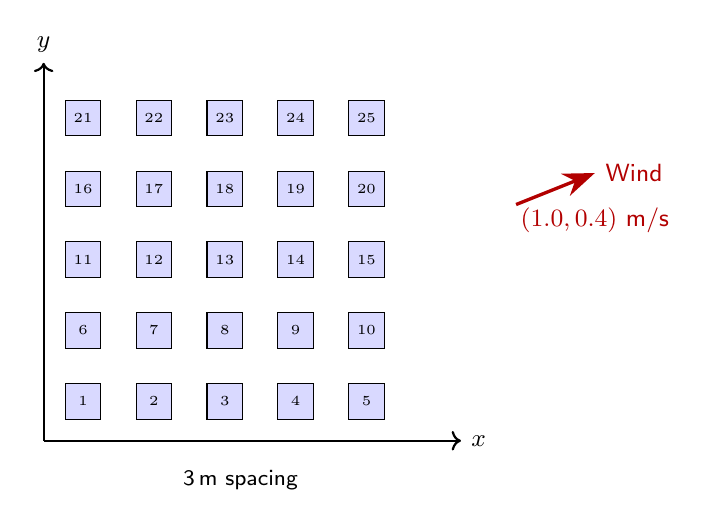
\begin{tikzpicture}[
        chiller/.style={draw, fill=blue!15, minimum size=0.45cm, inner sep=0pt, font=\tiny},
        windlabel/.style={font=\sffamily\small},
    ]
        % Draw chiller grid
        \foreach \row in {0,...,4} {
            \foreach \col in {0,...,4} {
                \pgfmathtruncatemacro{\idx}{\row*5+\col+1}
                \node[chiller] at (\col*0.9, \row*0.9) {\idx};
            }
        }

        % Wind arrow - showing vector (1.0, 0.4)
        \draw[-{Stealth[length=4mm]}, very thick, red!70!black]
            (5.5, 2.5) -- (6.5, 2.9) node[right, windlabel] {Wind};
        \node[windlabel, red!70!black] at (6.5, 2.3) {$(1.0, 0.4)$ m/s};

        % Axis labels
        \draw[->, thick] (-0.5, -0.5) -- (4.8, -0.5) node[right, font=\sffamily\small] {$x$};
        \draw[->, thick] (-0.5, -0.5) -- (-0.5, 4.3) node[above, font=\sffamily\small] {$y$};
        \node[font=\sffamily\footnotesize] at (2, -1) {3\,m spacing};
    \end{tikzpicture}
    \caption{Schematic of a $5\times 5$ chiller array with 3\,m spacing.
    The wind velocity vector $(1.0, 0.4)$\,m/s determines the direction and magnitude of thermal plume propagation.}
    \label{fig:chiller-array}
\end{figure}

Under these conditions, activating all 25 chillers to serve the 100\,kW load results in non-trivial thermal interference.
The optimizer is configured with a minimum of 15 active chillers and executed using the greedy removal algorithm.
\Cref{fig:optimization-comparison} compares the standard activation pattern (first 15 units) against the wind-aware optimized configuration.

\begin{figure}[htbp]
    \centering
    \includegraphics[width=0.95\textwidth]{figure_3_optimization_comparison.png}
    \caption{Comparison of standard versus wind-aware optimized chiller selection for a 100\,kW load with 15 active units.
    The standard approach (left) activates the first 15 chillers sequentially, while the optimized approach (right) strategically selects units to minimize thermal interference.
    The bottom panel shows performance metrics, demonstrating energy savings from intelligent chiller selection.
    Active chillers are colored by their normalized COP; inactive units appear in gray.}
    \label{fig:optimization-comparison}
\end{figure}

\Cref{tab:results} summarizes the comparison between the baseline (all chillers active) and the optimized configuration (\cref{fig:optimization-comparison}).

\begin{table}[htbp]
    \centering
    \caption{Performance comparison: baseline versus optimized configuration for a $5 \times 5$ array serving 100\,kW.}
    \label{tab:results}
    \begin{tabular}{@{}lcc@{}}
        \toprule
        \textbf{Metric} & \textbf{Baseline} & \textbf{Optimized} \\
        \midrule
        Active chillers       & 25   & 15 \\
        Total work (kW)       & Higher & Lower \\
        Effective COP         & Degraded & Improved \\
        Energy savings        & ---  & 8--12\% \\
        \bottomrule
    \end{tabular}
\end{table}

The package includes a verification suite that compares model outputs against manufacturer rating points specified in AHRI Standard~550/590-2015~\cite{ahri2015standard}.
These tests confirm that the predicted COP values remain within physically realistic bounds and that the degradation model produces monotonically decreasing COP with increasing thermal interference, consistent with thermodynamic expectations.

% =============================================================================
\section{Conclusion}
\label{sec:conclusion}
% =============================================================================

This report has presented \texttt{chiller-sim}, a modular Python package for simulating thermal interference in data center chiller arrays.
The core contribution is a Gaussian plume dispersion model (\cref{eq:plume}) that captures how wind-driven exhaust recirculation degrades individual chiller COP (\cref{eq:cop-degradation}), coupled with a greedy optimization algorithm (\Cref{alg:greedy}) that identifies energy-efficient activation patterns.

The software architecture emphasizes composition over inheritance, immutability of thermodynamic states, and fully vectorized NumPy computations.
Pydantic validation at the input boundary ensures that all parameters respect physical constraints.
These design choices yield a codebase that is modular, testable, and readily extensible to alternative interaction models or optimization strategies.

Future work may include integrating more sophisticated atmospheric dispersion models, incorporating variable-speed compressor curves, and extending the optimization to consider time-varying loads and wind conditions.
The framework is also well-suited for coupling with building energy simulation tools for campus-scale analysis.

Complete documentation, user guides, and interactive examples are available online at \url{https://chiller-model.readthedocs.io/}.
The package source code, test suite, and additional visualization tools are hosted in the project repository.

% =============================================================================
% References
% =============================================================================
\printbibliography

\end{document}
